\chapter{SYSTEM DESIGN AND IMPLEMENTATION}
\label{chap:caseFarming}

This chapter describes the implementation of the system which consists of two subsystems: A crowd-sourcing system and an analysis system. In \textit{Requirement analysis and System overview} subsection, everything is briefly described as a whole. In two last sections, structure and details of two subsystems are defined more comprehensively.

\section{Requirement analysis and system overview}
\subsection{Requirement analysis}

Figure \ref{chap3:system_overview_basic} shows a concise overview of how the system operates. Users interact with the website through \textbf{User Interfaces}. The input of users can come in the form of images, videos or label contribution and are stored in the database. The system is also responsible for obtaining appropriate contents from the database to display to users through user interfaces.

\begin{center}
    \begin{figure}[H]
    \centering
    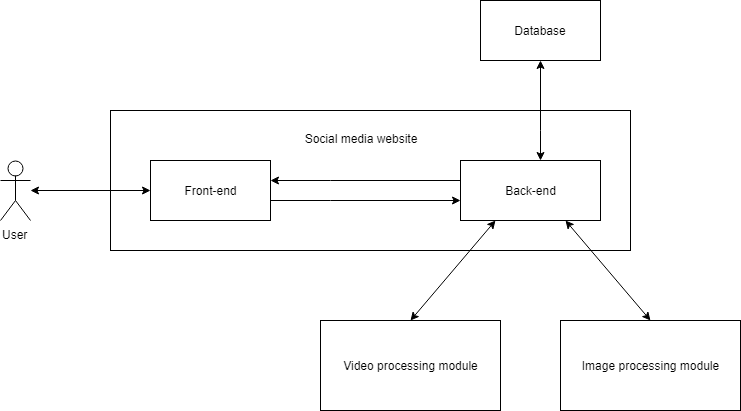
\includegraphics[width=1\columnwidth]{images/chap3/system_overview_basic.png}
    \caption{An overview of the system}
    \label{chap3:system_overview_basic}
    \end{figure}
\end{center}

Whenever there are videos to analyze, the server will send them to the \textbf{Video classifier module}, then get results back. Results returned from video classifier module are classified activity from the video and frames that contain faces in them. \textbf{Face Recognition module} does the job of identifying people in images. Results of both \textbf{Video classifier module} and \textbf{Face Recognition module} are used to determine security threats each video or image shows.
\section{Crowd-sourcing system}
\subsection{Database}
The project database divides into two different parts: \textbf{Cloud storage} and a \textbf{NoSQL database}. Why it requires such a complex system? The primary target is to reduce website loading time. Let take an example, if files are stored directly on the crowd-sourcing server. When many users request a file simultaneously, the server with limited bandwidth will cause delay. “53\% of mobile site visitors leave a page that takes longer than three seconds to load” – \href{https://think.storage.googleapis.com/docs/mobile-page-speed-new-industry-benchmarks.pdf}{Google}. What if these files stored on cloud storage? The client will be served by the cloud storage provider, which has higher availability.
\section{Analysis system}
The project requires two systems for analysis: A face recognition system and a video classifier system. The facial recognition system takes pictures of human faces as input and returns their identification. The video classifier system analyzes videos to find out actions in them. The remaining of this section describes in detail about the two analysis system.
\subsection{Face recognition module}
\subsection{Video classifier module}
Video classifying is not a new task in the field of Deep learning.
	
